\documentclass[
version=last,toc=bib,toc=graduated,toc=index,toc=listof,9pt,openany]{scrbook}
%\pdfminorversion=4
\usepackage{polyglossia}
\setdefaultlanguage{english}

\setmainfont{Source Sans Pro}
\setsansfont{Source Sans Pro}

\usepackage{ifmtarg}
\usepackage{ifthen}
\usepackage{etoolbox} % \ifstrempty

\usepackage{geometry}
\geometry{%a6paper
paperwidth=125mm, paperheight=168mm, 
portrait,
top=22mm, inner=22mm, outer=20mm, bottom=25mm,
headsep=3mm, footskip=12mm
}

\usepackage{ragged2e} % nicer typesetting (hyphenation) for non raggedright and raggedleft
\usepackage{lscape}
\setlength{\parskip}{0pt}

\usepackage{relsize}

\clubpenalty=10000
\widowpenalty=10000 
\displaywidowpenalty=10000

\usepackage[letterspace=16]{microtype}

\usepackage{graphicx} % graphics

% search path for images
\graphicspath{{images-print/}{icons/}{extra-pages/}{wallpaper/}}
\usepackage{wrapfig}  % sponsor logos wrapped with text

\usepackage{tabu}
\usepackage{tabularx}
\usepackage{longtable}
\usepackage[table,cymk]{xcolor}
\usepackage{colortbl}

% embed PDF pages
% pdfpages must not be loaded before colortbl!
\usepackage{pdfpages}

\usepackage{multirow}
\usepackage{booktabs}
\usepackage{array}

\usepackage{refcount} % calculation of the page where the map is located

% page background
\usepackage[manualmark]{scrlayer-scrpage}
\pagestyle{scrplain}

\newcommand{\acro}[1]{{\textsmaller{#1}}} % macro for abbreviations with more than one capitalised letter


% title/metadata
\title{State of the Map 2018}
\subtitle{Programme}
\author{OpenStreetMap Foundation}
\date{\today}

\clearscrheadings

% page numbers
\cfoot[\begin{small}\pagemark\end{small}]{\begin{small}\pagemark\end{small}}
\ofoot[]{}
\ifoot[]{}
\pagestyle{scrplain}

\linespread{1.15}

% include our custom macros
% command for a new time slot
\newcommand{\talktime}{9:99}
\newcommand{\newtimeslot}[1]{\newpage\renewcommand{\talktime}{#1}}

% new time slot but without a pagebreak
\newcommand{\newsmalltimeslot}[1]{\renewcommand{\talktime}{#1}}

% initialise \conferenceDay 
\newcommand{\conferenceDay}{Noday}


% define default page style (cutting marks with page number)
\DeclareNewLayer[background, oddorevenpage, width=125mm,%
height=169mm, contents={%
  
\includegraphics{wallpaper/crop-marks.pdf}%
}]{cropmarksevery}
\newpairofpagestyles[scrheadings]{cropmarksstyle}{}
\AddLayersAtBeginOfPageStyle{cropmarksstyle}{cropmarksevery}

% page style for title pages
\DeclareNewLayer[background, oddorevenpage, width=125mm,%
height=169mm, contents={%
  
\includegraphics{wallpaper/front-cover-with-crop-marks.pdf}%
}]{titlelayer}
\newpairofpagestyles[]{titlestyle}{}
\AddLayersAtBeginOfPageStyle{titlestyle}{titlelayer}

% define alias commands for all three days
\def\saturday{Saturday}
\def\sunday{Sunday}
\def\monday{Monday}

% define Saturday page style
\DeclareNewLayer[background, oddpage,  width=125mm,%
height=169mm, contents={%
  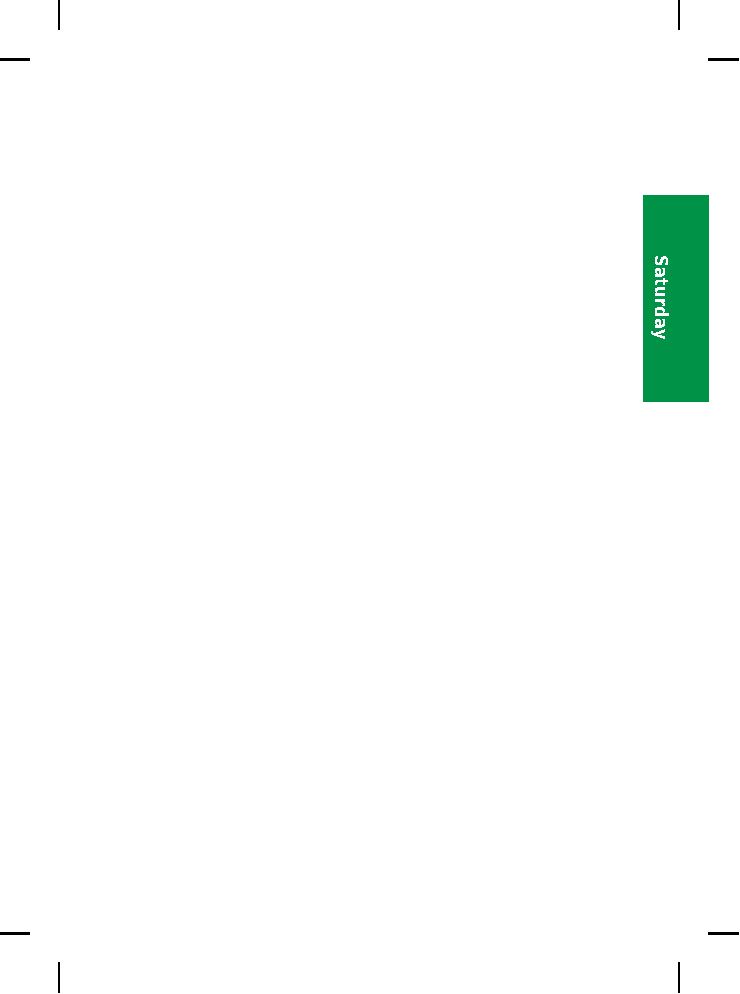
\includegraphics{wallpaper/saturday-odd.pdf}%
}]{saturdayodd}
\DeclareNewLayer[background, evenpage,  width=125mm,%
height=169mm, contents={%
  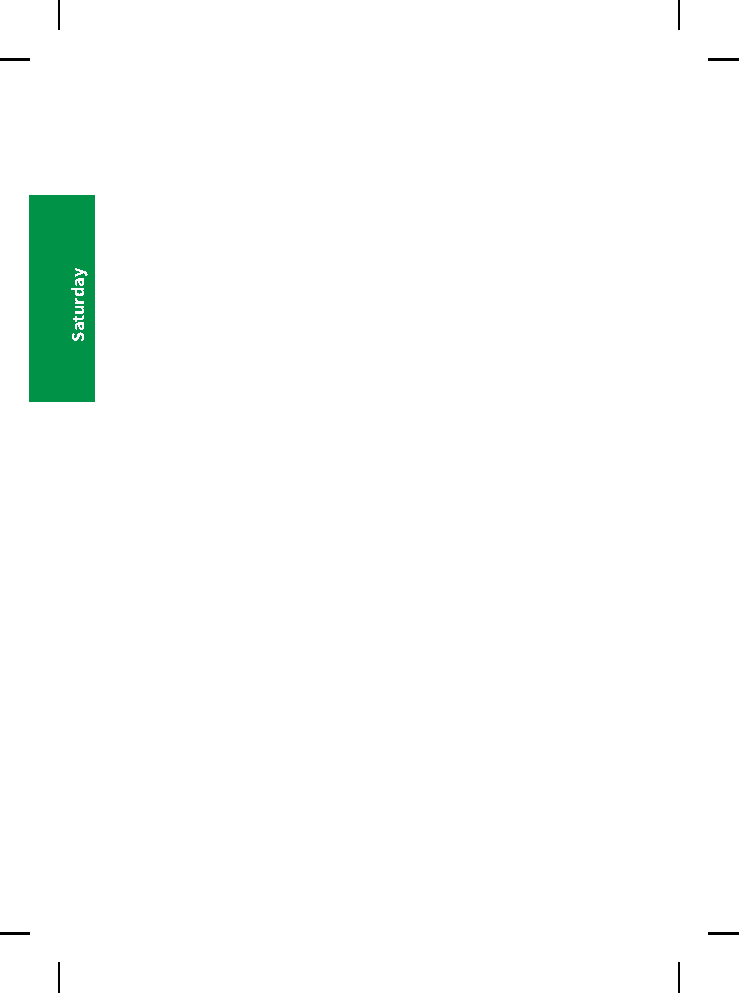
\includegraphics{wallpaper/saturday-even.pdf}%
}]{saturdayeven}
\DeclareNewLayer[background, oddpage,  width=125mm,%
height=169mm, contents={%
  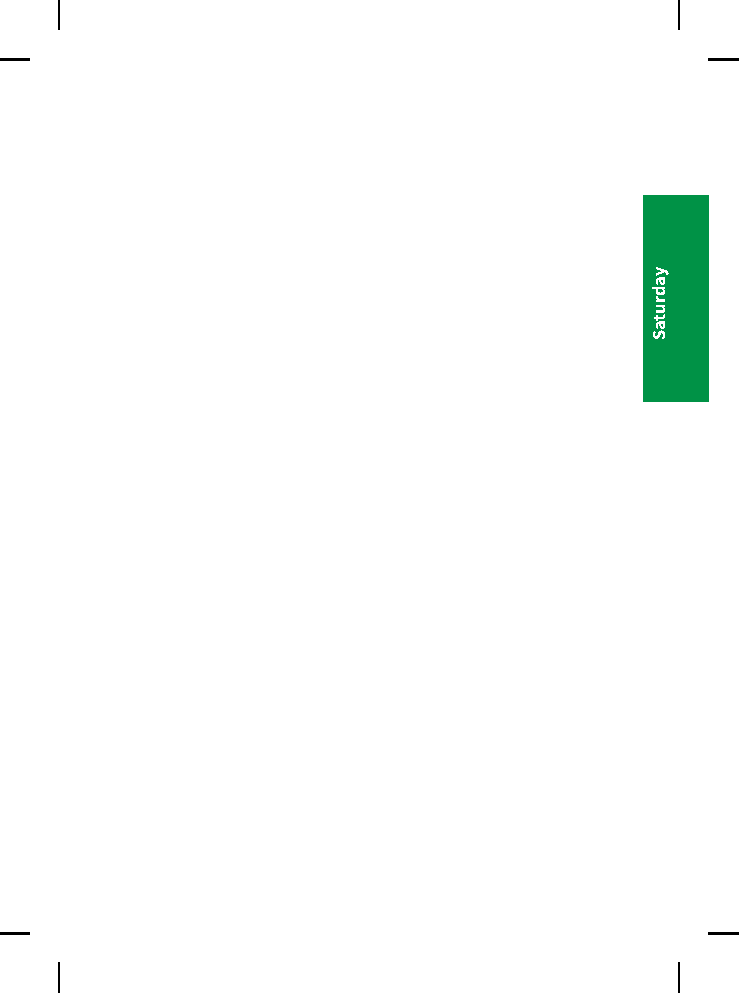
\includegraphics{wallpaper/saturday-odd-rotated.pdf}%
}]{saturdayoddrotated}
\newpairofpagestyles[scrheadings]{saturday-table}{}
\AddLayersAtBeginOfPageStyle{saturday-table}{saturdayeven}
\AddLayersAtBeginOfPageStyle{saturday-table}{saturdayoddrotated}
\newpairofpagestyles[scrheadings]{saturday}{}
\AddLayersAtBeginOfPageStyle{saturday}{saturdayeven}
\AddLayersAtBeginOfPageStyle{saturday}{saturdayodd}

% define Sunday page style
\DeclareNewLayer[background, oddpage,  width=125mm,%
height=169mm, contents={%
  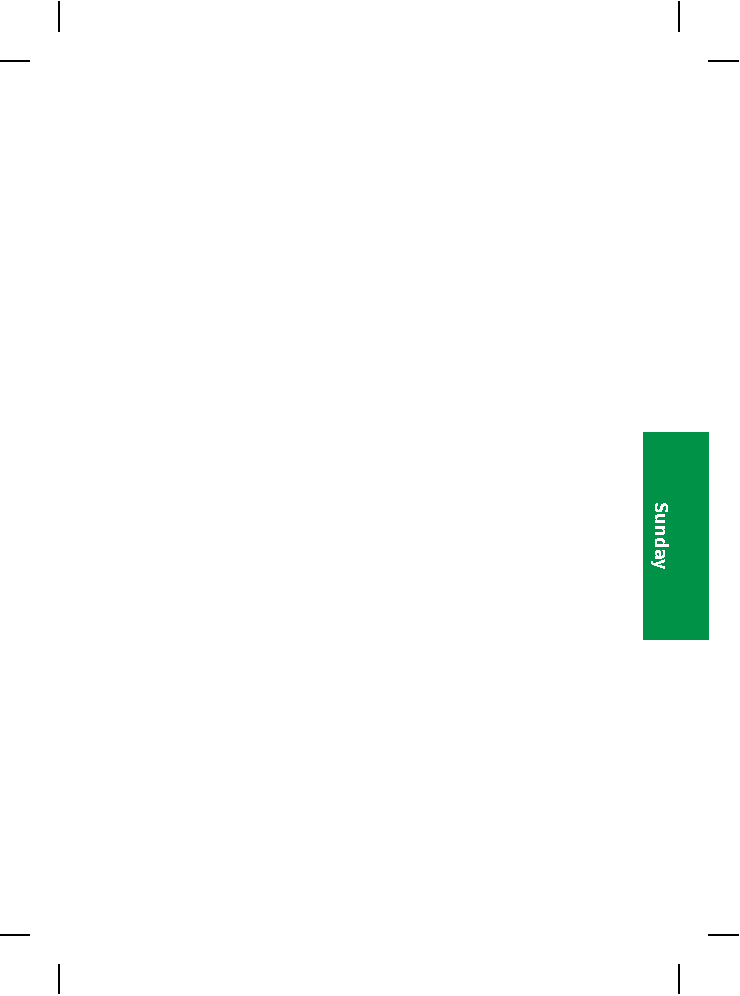
\includegraphics{wallpaper/sunday-odd.pdf}%
}]{sundayodd}
\DeclareNewLayer[background, evenpage,  width=125mm,%
height=169mm, contents={%
  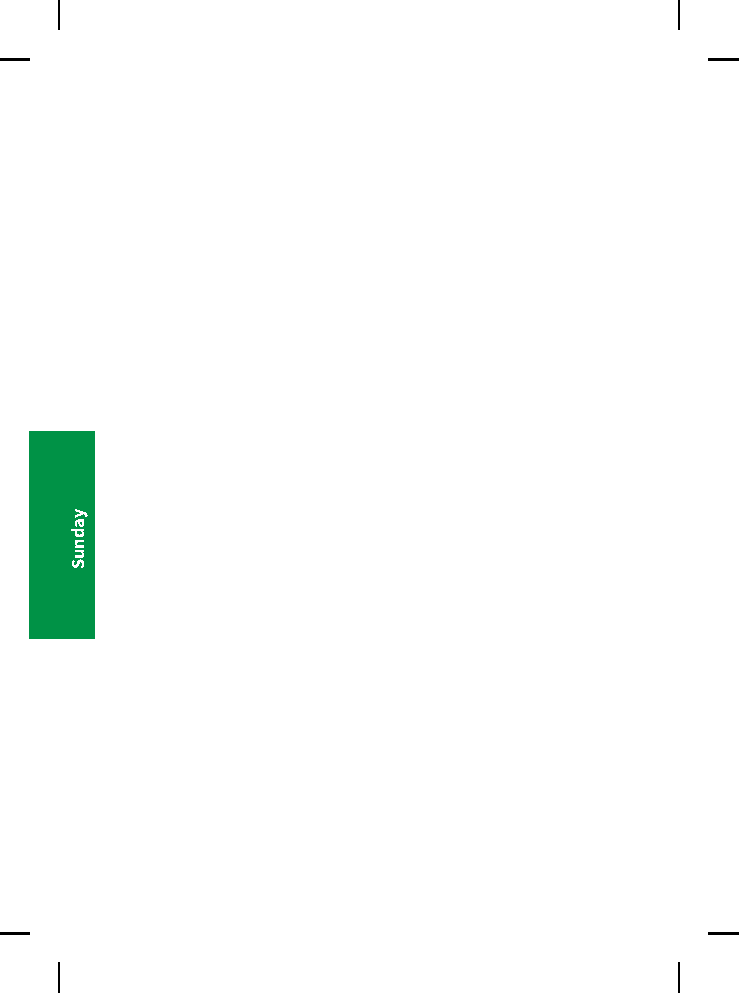
\includegraphics{wallpaper/sunday-even.pdf}%
}]{sundayeven}
\DeclareNewLayer[background, oddpage,  width=125mm,%
height=169mm, contents={%
  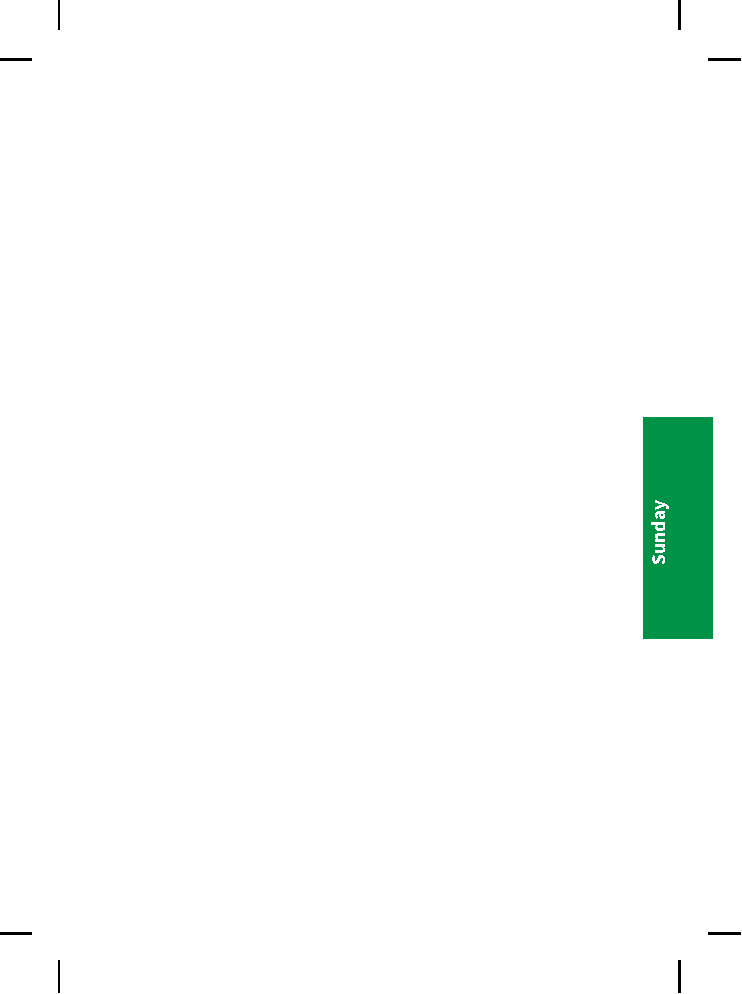
\includegraphics{wallpaper/sunday-odd-rotated.pdf}%
}]{sundayoddrotated}
\newpairofpagestyles[scrheadings]{sunday-table}{}
\AddLayersAtBeginOfPageStyle{sunday-table}{sundayeven}
\AddLayersAtBeginOfPageStyle{sunday-table}{sundayoddrotated}
\newpairofpagestyles[scrheadings]{sunday}{}
\AddLayersAtBeginOfPageStyle{sunday}{sundayeven}
\AddLayersAtBeginOfPageStyle{sunday}{sundayodd}

% define Monday page style
\DeclareNewLayer[background, oddpage,  width=125mm,%
height=169mm, contents={%
  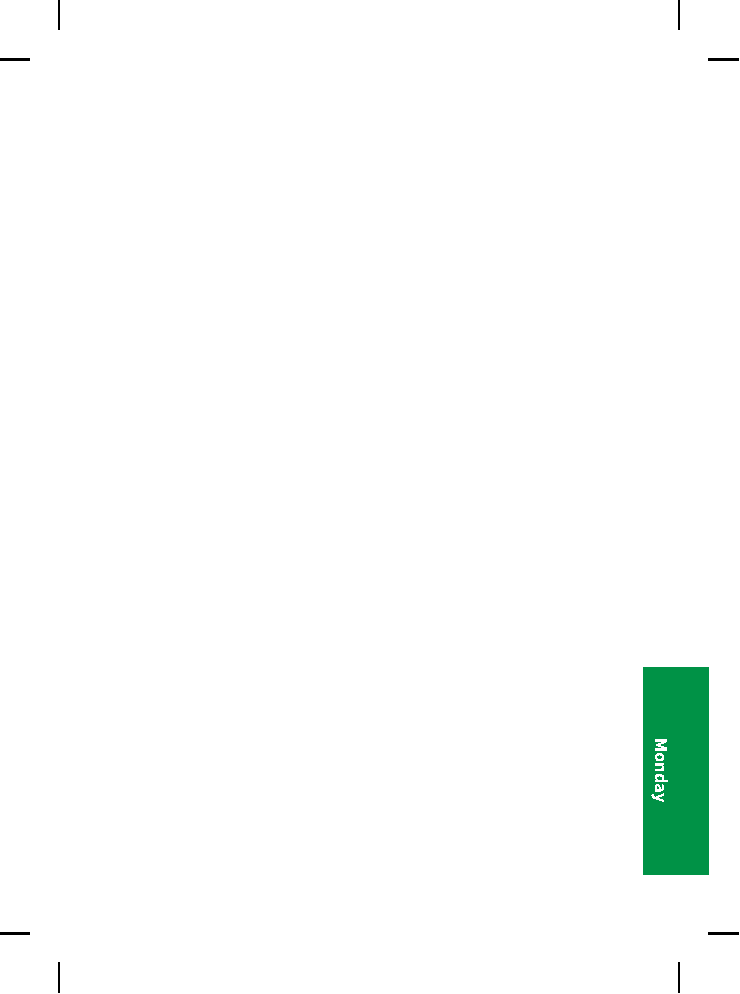
\includegraphics{wallpaper/monday-odd.pdf}%
}]{mondayodd}
\DeclareNewLayer[background, evenpage,  width=125mm,%
height=169mm, contents={%
  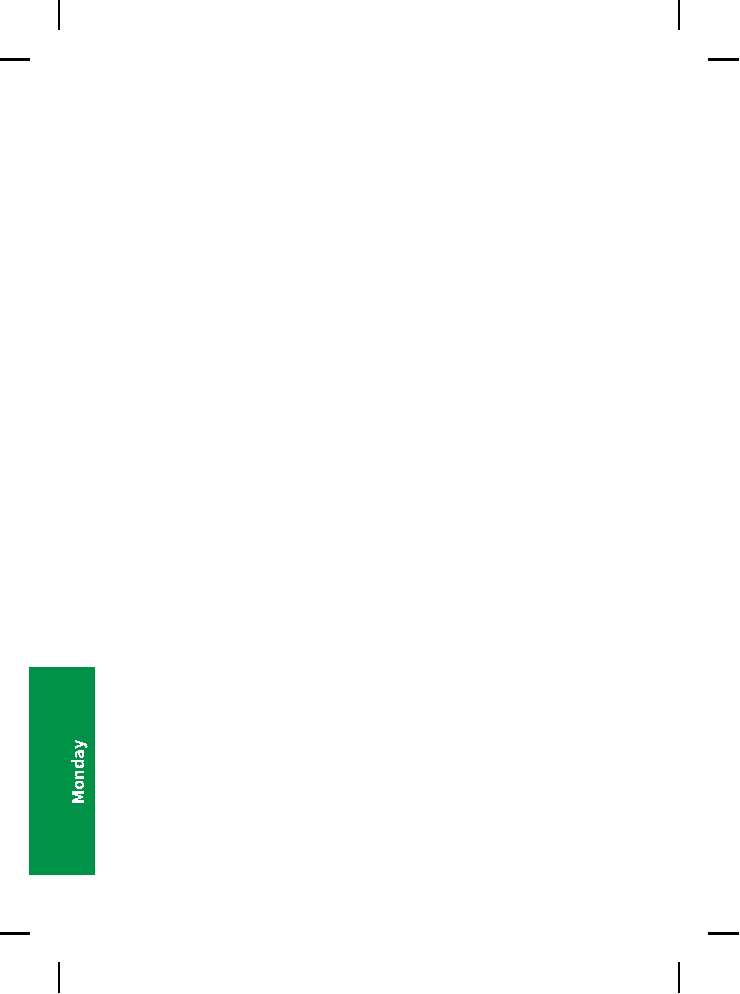
\includegraphics{wallpaper/monday-even.pdf}%
}]{mondayeven}
\DeclareNewLayer[background, oddpage,  width=125mm,%
height=169mm, contents={%
  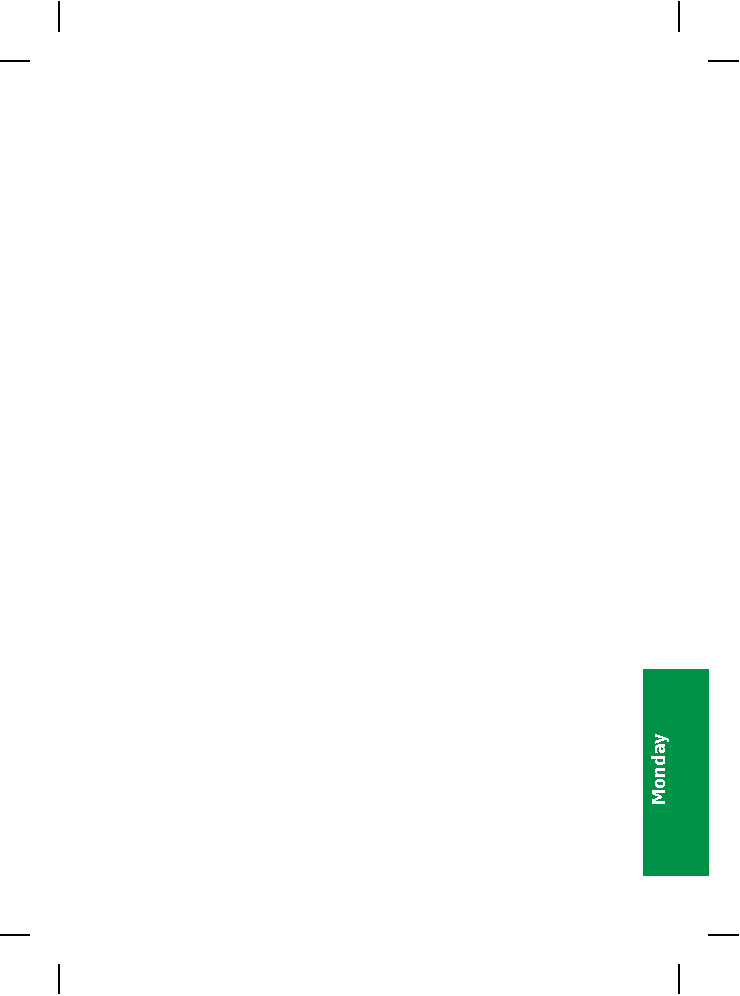
\includegraphics{wallpaper/monday-odd-rotated.pdf}%
}]{mondayoddrotated}
\newpairofpagestyles[scrheadings]{monday-table}{}
\AddLayersAtBeginOfPageStyle{monday-table}{mondayeven}
\AddLayersAtBeginOfPageStyle{monday-table}{mondayoddrotated}
\newpairofpagestyles[scrheadings]{monday}{}
\AddLayersAtBeginOfPageStyle{monday}{mondayeven}
\AddLayersAtBeginOfPageStyle{monday}{mondayodd}

% \setpagebackground selects the page style to be used depending on the current day. Each day has
% its own page style.
\newcommand{\setpagebackground}{ %
  \ifthenelse{\equal{\conferenceDay}{\saturday}}{%
    \pagestyle{saturday}
  }{}
  \ifthenelse{\equal{\conferenceDay}{\sunday}}{%
    \pagestyle{sunday}
  }{}
  \ifthenelse{\equal{\conferenceDay}{\monday}}{%
    \pagestyle{monday}
  }{}
}


% additional column type for tables
\newcolumntype{Y}[1]{>{\RaggedRight\arraybackslash}p{#1}}

%% length of the title boxes
\newlength{\titleboxwidth}
\setlength{\titleboxwidth}{\textwidth}
\advance\titleboxwidth by -6pt

% command to lay out the title boxes
\newcommand{\setabstract}[6]{
	% 1. speaker
	% 2. title
	% 3. subtitle
	% 4. abstract (Text)
	% 5. colour
	% 6. room
	%\thispagestyle{scrheadings}
  \setpagebackground
	\setlength\tabcolsep{0pt}
	% \setlength{\fboxsep}{0pt}
	\noindent\fcolorbox{white}{#5}{\parbox{\titleboxwidth}{%
		\noindent\begin{tabu}{X[5L]r}
			\isspeakerempty{#1}{#2}{#6}
			\issubtitleempty{#3}
		\end{tabu}%
	}}
	%
	\isabstractempty{#4}%
	\vspace{0.5em}% space to the next talk even if there is no abstract
	\setlength\tabcolsep{6pt} % set column padding back to default value
}

% lay out the speaker if there is any
% We assume that there is only a subtitle if the talk has a speaker.
\makeatletter
\newcommand{\isspeakerempty}[3]{%
	% Arguments:
	% 1. speaker
	% 2. title
	% 3. room
	\@ifmtarg{#1}{%
			\par\noindent\large \sectfont #2% % titel
			&
			#3, \talktime
			\tabularnewline
		}
		{
			\emph{#1} % Sprecher
			&
			\talktime
			\tabularnewline
			{\par\noindent\large \sectfont #2}% % titel
			&
			#3
			\tabularnewline
		}
		
}
\makeatother

% Lay out the subtitle
% has to be a separate function and has to be surrounded by \makeatletter for technical reasons
\makeatletter
\newcommand{\issubtitleempty}[1]{%
	\@ifnotmtarg{#1}{\multicolumn{2}{Y{\linewidth}}{\vspace{-0.6em} \noindent\bfseries \normalsize \sectfont #1}\tabularnewline}
}
\makeatother

% Lay out the abstract if there is any
% has to be a separate function and has to be surrounded by \makeatletter for technical reasons
\makeatletter
\newcommand{\isabstractempty}[1]{%
  \ifstrempty{#1}{%
    \vspace{1.5em}%
  }{%
    \vspace{0.5em}\newline%
    #1 \par% % abstract
    \vspace{1.5em}% space to the next talk even if there is an abstract
  }%
}
\makeatother

% define colours
\definecolor{deDonato}{cmyk}{0.16 0 .05 0}
\definecolor{two}{cmyk}{0.02 0 0.12 0.11}
\definecolor{academic}{cmyk}{0 0.02 0.23 0}
\definecolor{four}{cmyk}{0.35 0 0.33 0.16}
\definecolor{lightred}{cmyk}{0 .24 0.29 .04}

% session at De Donato
\newcommand{\abstractDeDonato}[4]%
{%
	\setabstract{#1}{#2}{#3}{#4}{deDonato}{De Donato}
}

% abstract at S.0.3
\newcommand{\abstractTwo}[4]%
{%
	\setabstract{#1}{#2}{#3}{#4}{two}{S.0.3}
}

% abstract at S.1.3
\newcommand{\abstractAcademic}[4]%
{%
	\setabstract{#1}{#2}{#3}{#4}{academic}{S.1.3}
}

% abstract at S.1.5
\newcommand{\abstractFour}[4]%
{%
	\setabstract{#1}{#2}{#3}{#4}{four}{S.1.5}
}

% abstract at a different location
\newcommand{\abstractOther}[5]%
{%
	\setabstract{#1}{#2}{#3}{#4}{commongray}{#5}
}

% box for workshops (they don't have an abstract in the booklet)
\newcommand{\workshopbox}[3]%
{%
	% 1. titel
	% 2. speaker
	% 3. Room
	\setlength\tabcolsep{0pt}
	\noindent\fcolorbox{white}{lightred}{\parbox{\titleboxwidth}{%
			\noindent
			\begin{tabu}{X[5L]r}
				\emph{#2} % speaker
				&
				\talktime
				\tabularnewline
				{\noindent\large \bfseries #1}% % title
				&
				#3
				\tabularnewline
			\end{tabu}
		}
	}
	\setlength\tabcolsep{6pt} % set column padding back to default
}

% too long
\newcommand{\tooLong}{Dieser Text ist viel zu lang. Dieser Text ist viel zu lang. Dieser Text ist viel zu lang. Dieser Text ist viel zu lang. Dieser Text ist viel zu lang. Dieser Text ist viel zu lang. Dieser Text ist viel zu lang. Dieser Text ist viel zu lang. Dieser Text ist viel zu lang. Dieser Text ist viel zu lang. Dieser Text ist viel zu lang. Dieser Text ist viel zu lang. Dieser Text ist viel zu lang. Dieser Text ist viel zu lang. }

\newlength{\fboxwidth}

\def\workshopsSection{workshopsSection}
\def\abstractsSection{abstractsSection}

% boxes for text-only advertisement texts by our sponsors
\newcommand{\sponsorenbox}[4]{%
  \setlength{\fboxwidth}{\textwidth}
  \advance\fboxwidth by -7.0pt
  \abstractSponsorenbox{#1}{#2}{#3}{#4}{\workshopsSection}%
}

\newcommand{\sponsorenboxA}[4]{%
  \setlength{\fboxwidth}{\textwidth}
  \advance\fboxwidth by -10.0pt
  \abstractSponsorenbox{#1}{#2}{#3}{#4}{\abstractsSection}%
}

%% box for advertisment by a sponsor
%% 1. logo
%% 2. width of the logo
%% 3. number of required lines of the logo (due to usage of wrapfigure)
%% 4. text
%% 5. Umfeld (\workshopsSection oder \abstractsSection}
\makeatletter
\newcommand{\abstractSponsorbox}[5]{%
  \setlength{\fboxsep}{4.5pt}%
  \noindent%
  \ifthenelse{\equal{#5}{\workshopsSection}}{%
    \hspace{2.65pt}%
  }{%
    \hspace{-1pt}%
  }%
  \fcolorbox{gray}{white}{%
    \parbox{\fboxwidth}{
    \@ifmtarg{#1}{}{%
      \begin{wrapfigure}[#3]{r}[0pt]{#2}
        \centering\vspace{-1\baselineskip}
        \includegraphics[width=#2]{#1}
      \end{wrapfigure}
    }

    \noindent #4
    }%
  }
  \setlength{\fboxsep}{3pt}
}
\makeatother

% definition of column types for the schedule tables
\newcolumntype{Z}[1]{>{\RaggedRight\arraybackslash}p{#1}}%
\newcolumntype{C}[1]{>{\Centering\arraybackslash}p{#1}}%

% common implementation of typesetting of a session in the tables
\newcommand{\talkInternal}[2]{%
  \textbf{#1}
  \ifthenelse{\equal{#2}{}}{}{%
    \newline\emph{#2}%
  }
}

% macro to typeset a talk in the schedule tables spanning over more than one row:
% usage: \longTalk{rowcount}{title}{speaker}
\newcommand{\longTalk}[3]{%
  &
  \multirow{#1}{\linewidth}{%
    \parbox{\linewidth}{
      %HACK Inserting a \vspace here is a dirty hack but it works.
      \vspace{0.45\baselineskip}
      \talkInternal{#2}{#3}%
    }
  }%
}%

% macro to typeset a talk in the schedule tables spanning over more than one row:
% usage: \talk{title}{speaker}
\newcommand{\talk}[2]{%
  &
  \talkInternal{#1}{#2}%
}%


\newcommand{\workshop}[3]%
{%
	\workshopbox{#1}{#2}{#3}
}%

\newcommand{\otherevent}[1]%
{%
	& \textbf{#1}
}%

\newcommand{\aulaevent}[2]%
{%
	&
	\multicolumn{3}{c}{
		\textbf{#1} (Aula) \par \emph{#2}
	}
}%

\newcommand{\coffeespace}{\vspace{0.4em}}
\newcommand{\workshopspace}{\vspace{0.5em}\\}

% define colors
\definecolor{commongray}{gray}{.9}
\renewcommand{\arraystretch}{1.4}



\begin{document}
 
\pagestyle{cropmarksstyle}
\begin{titlepage}
  \thispagestyle{titlestyle}
  \null
\end{titlepage}
\pagestyle{cropmarksstyle}

\selectlanguage{english}
\section*{Content}

\vspace*{0.35em}%
\noindent Welcome\dotfill \pageref{welcome}

\vspace*{0.35em}%
\noindent Scholarships \dotfill \pageref{scholarships}

\vspace*{0.35em}%
\noindent Code of Conduct \dotfill \pageref{coc}

\vspace*{0.35em}%
\noindent Getting around in Milan\dotfill \pageref{getting-around}

\vspace*{0.35em}%
\noindent Saturday schedule\dotfill \pageref{saturday}

\vspace*{0.35em}%
\noindent Sunday schedule \dotfill \pageref{sunday}

\vspace*{0.35em}%
\noindent Monday schedule \dotfill \pageref{monday}

\vspace*{0.35em}%
\noindent Thank you \dotfill \pageref{thanks}

\vspace*{0.35em}%
\noindent Legal notice \dotfill \pageref{legal}

\vfill
\noindent
Hashtag: \#sotm

\vspace*{0.8em}%
\noindent
The general emergency telephone number in Italy is \textbf{112}.
\vfill

\newpage

\newpage
\section*{Welcome to Milan and to State of the Map 2018} \label{welcome}
This booklet gives you essential information
about the conference, the location and the schedule.  We are proud of the participation of the
OpenStreetMap community and our rich program but there is even more!  Please do get involved and
take advantage of the off-schedule sessions, discussions and spaces.

\paragraph*{The location} \label{welcome-location}
One room is available during the whole conference as free and open space offering chairs and tables
to talk to each other, work on your projects or just relax.  Two rooms are available for
self-organised sessions.  See page~\pageref{self-organised} for further information.  A floor plan
of the building can be found on page~\pageref{floorplan}.

\paragraph*{Help desk} \label{welcome-helpdesk}
You already know the registration desk, located at the ground floor (Building 3, same as the whole
conference).  It is also your port of call if you need support or help. We are listening to every
question, report and comment, related to the event, the code of conduct (page~\pageref{coc}) or any
aspect of the organisation.

\paragraph*{Sponsors} \label{welcome-sponsors}
We would like to thank our sponsors for making this event possible and for their support to the
OpenStreetMap Foundation.
\newpage

\newpage
\section*{Scholarships}
\label{scholarships}
\pagestyle{cropmarksstyle}

The OpenStreetMap Foundation is delighted to be able to provide scholarships to a number of
recipients from Europe, the Americas, Africa and Asia.

\begin{itemize}
  \setlength{\itemsep}{0pt}
  \item 12 full scholarships
  \item 4 enhanced scholarships
  \item 1 speaker grant
\end{itemize}

The selection committee consisted of the SotM Working Group supported by Heather Leson, Ilya Zverv,
Jóhannes Birgir Jensson, Maurizio Napolitano, Rebecca Firth, Sidorela Uku and Stefano Sabatini.

The OpenStreetMap Foundation was not the only organisation granting scholarships.  Les Libres
Geographes (LLG) with the overall support of Organisation Internationale de la Francophonie (OIF)
facilitates 5 scholarships. Wikimedia Deutschland faciliates some scholarships for Germans.

\section*{Getting around in Milan}
\label{getting-around}
\pagestyle{cropmarksstyle}
Azienda Trasporti Milanesi (ATM) operates a public transport network in Milan. Single tickets cost
€~1.50 and are available from newsstands, tobacconists (tabaccherie), bars and automatic ticket
machines in metro stations. 24\,h (€~4.50) and 48\,h (€~8.25) tickets, as well as a \emph{carnet} of 10 single
trips (€~13.80) are also available. An evening ticket (€~3.00) allows unlimited travel after 20:00.

Tickets should be stamped at the start of every journey and every time you change vehicles. To stamp
your ticket insert it into the slot in the electronic ticket machine on board overground vehicles or
at the ticket barriers in the metro. It is then valid for 90 minutes unlimited use (bus or tram), or
the completion of your full metro journey. Tickets are not sold on board and you will not find a
self-service ticket machine at bus and tram stop.

\section*{Code of Conduct}
\label{coc}
The OSM Foundation is dedicated to providing a harassment-free
conference experience for everyone, regardless of gender, gender identity
and expression, sexual orientation, disability, physical appearance, body
size, race, age or religion. We do not tolerate harassment of conference
participants in any form. Sexual language and imagery is not appropriate
for any conference venue, including talks.

Conference participants violating these rules may be sanctioned or
expelled from the conference without a refund at the discretion of the
conference organizers.

Our anti-harassment policy can be found on our website.

\newpage
\renewcommand{\arraystretch}{1.4}
\section*{Saturday Schedule}\label{saturday}
\renewcommand{\conferenceDay}{\saturday}
\setpagebackground
\begin{center}
  \noindent\begin{tabular}{Z{0.75cm}Z{6.85cm}}
    \cellcolor{commongray}
    &
    \multicolumn{1}{c}{
      \cellcolor{deDonato}
      De Donato
    }
    \tabularnewline
    \cellcolor{commongray}
    9:30
    \talk{Welcome}{}
    \tabularnewline
    \cellcolor{commongray}
    10:00
    \talk{Keynote OpenStreetMap—Now and into the Future}{Kate Chapman, Heather Leson}
    \tabularnewline
    \rowcolor{commongray}
  \end{tabular}

  \vspace{1.5\baselineskip}
  \noindent\begin{tabular}{Z{0.75cm}Z{3.0cm}Z{3.0cm}}
    \cellcolor{commongray}
    &
    \multicolumn{1}{c}{\cellcolor{deDonato} De Donato}
    & \multicolumn{1}{c}{\cellcolor{two} S.0.2}
    \tabularnewline
    \cellcolor{commongray}
    10:30
    \talk{Can we validate every change on OSM?}{Lukas Martinelli}
    \talk{Making Maps Without Databases}{Thomas Skowron}
    \tabularnewline
    \rowcolor{commongray}
    11:00 & \multicolumn{2}{c}{%
      \parbox[c]{24pt}{%
        
\includegraphics[height=10pt]{cafe}%
      }
      break} \tabularnewline
  \end{tabular}
\end{center}
  
\begin{center}
  \renewcommand{\arraystretch}{1.3}
  \noindent\begin{tabular}{Z{0.75cm}Z{2.0cm}Z{2.0cm}Z{2.0cm}}
    \cellcolor{commongray}
    & \multicolumn{1}{c}{\cellcolor{deDonato} De Donato}
    & \multicolumn{1}{c}{\cellcolor{two} S.0.3}
    & \multicolumn{1}{c}{\cellcolor{four} S.1.5}
    \tabularnewline
    \cellcolor{commongray}
    11:30
    \talk{Interpreting Imagery for OpenStreetMap}{Chad Blevins}
    \talk{OpenMapTiles: Vector tiles from OpenStreetMap}{Petr Pridal, Jiri Komarek}
    \talk{Qt to create Maps}{Paolo Angelelli}
    \tabularnewline
  \end{tabular}
\end{center}
  
\begin{center}
  \renewcommand{\arraystretch}{1.3}
  \noindent\begin{tabular}{Z{0.75cm}Z{2.0cm}Z{2.0cm}Z{2.0cm}}
    \cellcolor{commongray}
    & \multicolumn{1}{c}{\cellcolor{deDonato} De Donato}
    & \multicolumn{1}{c}{\cellcolor{two} S.0.3}
    & \multicolumn{1}{c}{\cellcolor{four} S.1.5}
    \tabularnewline
    \cellcolor{commongray}
    12:00
    %\talk{Advertising mapping: using OpenStreepMap for the protection of landscape}{Paul Desgranges}
    \talk{Advertising mapping}{Paul Desgranges}
    \talk{Large Scale Deep Learning for Map Making}{Alina Negreanu and Bogdan Gliga}
    \talk{Field Mapping tools and technologies}{Paul Uithol}
    \tabularnewline
    \cellcolor{commongray}
    12:30
    \talk{An excursion in to the world of OSM tagging presets}{Simon Poole}
    \talk{How Deep Learning could help to improve OSM Data Quality?}{Oliver Courtin}
    \tabularnewline
    \rowcolor{commongray}
    13:00 & \multicolumn{3}{c}{%
    \parbox[c]{24pt}{%
      
\includegraphics[height=10pt]{restaurant}%
    }
    lunch} \tabularnewline
    \rowcolor{commongray}
    14:00
    & \multicolumn{3}{c}{photo}
    \tabularnewline
    \cellcolor{commongray}
    14:10
    \talk{Addressing addresses}{Sarah Hoffmann}
    % \talk{The Belgian perspective to building OpenStreetMap community}{Ben Abelshausen, Joost Schouppe}
    \talk{Belgian perspective to building OSM community}{Ben Abels\-hausen, Joost Schouppe}
    \talk{Lightning Talks 1}{}
    \tabularnewline
  \end{tabular}
\end{center}
  
\begin{center}
  \renewcommand{\arraystretch}{1.3}
  \noindent\begin{tabular}{Z{0.75cm}Z{2.0cm}Z{2.0cm}Z{2.0cm}}
    \cellcolor{commongray}
    & \multicolumn{1}{c}{\cellcolor{deDonato} De Donato}
    & \multicolumn{1}{c}{\cellcolor{two} S.0.3}
    & \multicolumn{1}{c}{\cellcolor{four} S.1.5}
    \tabularnewline
    \cellcolor{commongray}
    14:40
    \talk{2, 4, 6, 8, Here's how we interpolate}{Julian Simioni}
    % \talk{A new approach to garner prolific contribution in OpenStreetMap}{Kshitiz Khanal}
    \talk{New approach to garner prolific contribution in OSM}{Kshitiz Khanal}
    \talk{The LWG Presents: GDPR Implementation for OSM}{Kathleen Lu}
    \tabularnewline
    \cellcolor{commongray}
    15:10
    \talk{OsmAnd making live maps update}{Victor Shcerb}
    \talk{Building up the Microsoft Open Maps Team}{Osin Herriott}
    \tabularnewline
    \rowcolor{commongray}
    15:40
    & \multicolumn{3}{c}{%
    \parbox[c]{24pt}{%
      
\includegraphics[height=10pt]{cafe}%
    }
    break} \tabularnewline
    \cellcolor{commongray}
    16:10
    \talk{Lies, damned lies, and OSM statistics}{Frederik Ramm}
    \talk{Verifying Our Edits}{Bogdan Petrea, Armin Gheorghina}
    \talk{Corporate Cartography: How the sausage gets made}{Paul Norman}
    \tabularnewline
  \end{tabular}
\end{center}
  
\begin{center}
  \renewcommand{\arraystretch}{1.3}
  \noindent\begin{tabular}{Z{0.75cm}Z{2.0cm}Z{2.0cm}Z{2.0cm}}
    \cellcolor{commongray}
    & \multicolumn{1}{c}{\cellcolor{deDonato} De Donato}
    & \multicolumn{1}{c}{\cellcolor{two} S.0.3}
    & \multicolumn{1}{c}{\cellcolor{four} S.1.5}
    \tabularnewline
    \cellcolor{commongray}
    16:40
    \talk{An innovative approach to support OSM data generation}{Emanuela Mihut}
    \talk{Mapping Competition with Focus on Quality: Lesson Learned}{Yantisa Akhadi}
    \talk{Open Gender Monologues}{Heather Leson}
    \tabularnewline
    \cellcolor{commongray}
    17:10
    \talk{Pinpointing the power grid}{Sajjad Anwar}
    \talk{Improving OSMCha for the community}{Wille Marcel Lima Malheiro}
    \tabularnewline
    \rowcolor{commongray}
    19:30
    &
    \multicolumn{3}{c}{%
      \parbox[c]{24pt}{%
        
\includegraphics[height=10pt]{restaurant}%
      }%
      Social Event at Old Fashion Milano%
    }
    \tabularnewline
  \end{tabular}
\end{center}
\renewcommand{\arraystretch}{1.0}

\justifying
\newpage

\newsmalltimeslot{9:00}
% K001
% room: De Donato
% slot: 2
\abstractDeDonato{}%
{Welcome}%
{}%
{}

\newsmalltimeslot{9:30}
% K001
% room: De Donato
% slot: 2
\abstractDeDonato{Kate Chapman, Heather Leson}%
{OpenStreetMap—Now and into the Future}%
{}%
{%
  The beauty of OpenStreetMap is the variety of people contributing to the tapestry of the map.
  Those people have different backgrounds, motivations and reasons to contribute. We have come a
  long way from a few people meeting in person to a global community. While OSM is unique it does
  have a place amongst the other projects and organizations contributing in the open space. How do
  we fit into this place in the future? What parts of the path must we forge on our own and which
  can we learn from others? Does the project have a finite life cycle? How can we as a community
  think strategically to ensure we remain relevant? Let’s all continue to work together, now and
  into the future.%
}
% ------------------------------------

\newsmalltimeslot{10:00}
% T079
% room: De Donato
% slot: 3
\abstractDeDonato{Lukas Martinelli}%
{Can we validate every change on OSM?}%
{}%
{%
  OpenStreetMap receives 30,000 changesets everyday. Bad edits vary from novice mapping mistakes to
  intentional vandalism. Through Mapbox, hundreds of millions of users now view the map. Data
  quality has become crucial; we cannot afford to have our products affected by bad changes. We will
  present how we have built bulletproof protection against the daily vandalism we see.

  We will focus on what we have learned from our past approaches to catching vandalism. We will also
  discuss the creation of a new unit of change that scales better than both changesets and individual
  features. We have taken on the challenge of validating every edit to the map in the quickest time
  possible while only consuming upstream edits. In addition, we will explore how the community can
  join and benefit from our validation efforts.
  
  We are entering into an exciting new age for OSM with an unprecedented number of users consuming it
  daily, and we are excited to help protect the data quality of OpenStreetMap.%
}

% T092
% room: S.0.2
% slot: 3
\abstractTwo{Thomas Skowron}%
{Making Maps Without Database}%
{}%
{%
  The first step of processing OpenStreetMap data is loading it into a PostGIS database, only to
  retrieve all of it later on. This talk proposes strategies and tools to generate maps without
  using a database, which has performance benefits as well as better control about the result.%
}
% ------------------------------------

\newtimeslot{11:30}

% T076
% room: De Donato
% slot: 5
\abstractDeDonato{Chad Blevins}%
{Interpreting Imagery for OpenStreetMap}%
{}%
{%
  At one point or another every mapper has seen something on imagery that’s hard to distinguish from
  another feature, or is outright hard to describe.  Learning how your eyes and mind work together
  to interpret imagery is an art and something we can all practice.  This session will walk through
  examples of how you can associate imagery characteristics such as Shape, Size, Shadow, Time,
  Texture, and Pattern to help mappers improve their mapping skills, and improve OpenStreetMap.  %
}
% T065
% room: S.0.2
% slot: 5
\abstractTwo{Petr Pridal, Jiri Komarek}%
{OpenMapTiles: Vector tiles from OpenStreetMap}%
{}%
{%
  The OpenMapTiles is a free and open-source project, which makes it extremely easy to setup your
  own OpenStreetMap tileserver with vector and raster tiles. Design your own custom maps with an
  online editor or modify one of the beautiful open map styles. The maps are usable in web and
  mobile apps (with SDKs including Leaflet, OpenLayers, Mapbox), in desktop GIS tools and printed
  outputs.

  Learn how to adapt the schema and make your own vector tiles with a customized selection of
  OpenStreetMap tags or your own geodata - to display in the map the features you need - and how to
  contribute to the development of OpenMapTiles.
  
  The entire world turned into vector tiles fits on a USB disk - and can be hosted on any laptop, used
  offline, deployed on a regular hosting or on a private or public cloud. With Docker, you can run the
  maps in a few minutes on any infrastructure. We support open-source and open-data communities by
  offering forever free hosting on our global infrastructure.%
}
% T023
% room: S.1.5
% slot: 5
\abstractFour{Paolo Angelelli}%
{Qt to create OSM-based apps}%
{}%
{%
  The aim of the talk is to introduce the mighty Qt framework
  (https://en.wikipedia.org/wiki/Qt\_(software)) to the audience, then to drill down into its
  QtLocation module.  The goal is to demonstrate the functionalities of the module and of its
  OSM-backed plugins (osm, mapbox, mapboxgl) and how to easily pull together applications to do
  mapping, routing, geocoding and search places of interest with the power of QML and of
  OpenStreetMap.  These \emph{native} applications (as opposed to javascript-based or similar cross
  platform frameworks) can then be deployed everywhere thanks to the power of Qt. This means
  desktop, mobile and embedded platforms.%
}
% ------------------------------------

\newtimeslot{12:00}
% T017
% room: De Donato
% slot: 6
\abstractDeDonato{Paul Desgranges}%
{Advertising mapping: using OpenStreepMap for the protection of landscape }%
{}%
{%
%   Based on what I did recently in the use of OSM to map advertising devices (with the idea of protecting landscapes from the invasion of advertising):
%    - See 
%   https://wiki.openstreetmap.org/wiki/User:Barnes38#.282015.2F2017.29_Outdoor_advertising.2FPublicit.C3.A9_Ext.C3.A9rieure
%   - See  (French OpenData used in 2016 in cartography to figth against a french government decree project) https://wiki.openstreetmap.org/wiki/User:Barnes38#.28end_2015.2Fstart_2016.29_Cartography_for_Paysages_de_France
%   - Participation to French SOTM 2017 in Avignon (1h30 session) https://wiki.openstreetmap.org/wiki/User:Barnes38#.282_au_4_juin_2017.29_SOTM_France_in_Avignon
%   
%   I wish to make a summary of the OSM mapping specification (key : advertising), a summary of the way this key is used by OSM contributors worldwide, and to present new ideas to how to used OSM for protection of landscape.
% 
%   Thank you 
  % A version of the abstract written by Michael preserving the style but removing all the links which
  % are unclickable on paper.
  Based on what I did recently in the use of OSM to map advertising devices (with the idea of
  protecting landscapes from the invasion of advertising).  I wish to make a summary of the OSM
  mapping specification (key advertising), a summary of the way this key is used by OSM contributors
  worldwide, and to present new ideas to how to used OSM for protection of landscape.
%
}
% T115
% room: S.0.2
% slot: 6
\abstractTwo{Alina Negreanu and Bogdan Gliga}%
{Large Scale Deep Learning for Map Making}%
{}%
{%
  In this talk, the Telenav OSM team talks about what we have learned from our experience building a
  horizontally scalable deep learning pipeline that can process the >120 million images in the
  OpenStreetCam database. We will offer a technical perspective about how we used state of the art
  algorithms to detect a large number of traffic signs, extract road features like number of lanes
  visible on a road, and accurately perform text recognition on signs. This technology is now open
  source and available for anyone to use and improve upon!%
}
% W033
% room: S.1.5
% slot: 6
% slot: 7
\abstractFour{Paul Uithol}%
{Field Mapping tools \& technologies}%
{}%
{%
  If you want to get started on mapping things, be it data on schools, railway crossings, street
  names, or something entirely different, it's good to think about the tools you intend to use
  first. Especially if more people get involved! In this workshop, we'll demonstrate several topics
  related to data collection, and get some hands-on experience on:

  - Choosing what data to collect and why;
  - What data collection and mapping tool to use when, such as Maps.me, OpenDataKit, or OpenMapKit;
  - Creating a data model and forms;
  - Establishing baseline data; review existing data (OSM Analytics and other tools), review imagery, and set up digitization tasks with the Tasking Manager;
  - Collecting, reviewing, uploading and validating data;
  - (If time allows, more on logistics, safety and communications)

  The goal is to give an overview of several existing options and choices to make, and to get some
  hands-on experience with a couple of these tools!%
}
% ------------------------------------

\newtimeslot{12:30}
% T061
% room: De Donato
% slot: 7
\abstractDeDonato{Simon Poole}%
{An excursion in to the world of OSM tagging presets}%
{}%
{%
  Tagging presets have a large influence on how and in how much detail OSM contributors map.
  OpenStreetMap affords itself the luxury of multiple completely separate, independently developed
  preset systems.

  The talk investigates how different the systems are and how, if at all, this reflects in map data
  contributions.%
}
% T068
% room: S.0.2
% slot: 7
\abstractTwo{Olivier Courtin}%
{How Deep Learning could help to improve OSM Data Quality ?}%
{}%
{%
  How DeepLearning, and semantic segmentation, can be an efficient way to detect and spot
  inconsistency in OSM dataset ? 

  Machine and DeepLearning can succeed to tackle some old issues, in a far more convenient and
  efficient way than ever before… For instance DeepLearning, with aerial imagery semantic
  segmentation can improve features detection ability and allow us to spot dataset inconsistencies.
  
  In this presentation we will focus on how an OpenStreetMap subset dataset (for instance roads and
  buildings on an area), can be evaluated to produce quality metric.
  
  We wanna focus on:
  
  Deep Learning vision, and specific Satellite imagery considerations (high and low resolutions,
  multispectral dimensions, dataset aggregation…)
  
  How to qualify a good enough labelled DataSet (to allow supervised learning)
  
  FOSS4G (PostGIS and Grass) integration with Python ML/DL framework
  
  Concrete solution for efficient treatments for wide coverages%
}

% ------------------------------------

\newtimeslot{14:10}
% T094
% room: De Donato
% slot: 9
\abstractDeDonato{Sarah Hoffmann}%
{Addressing addresses}%
{}%
{%
  We are all used to describe locations with words. The concept is universally known as addresses.
  You put them on postcards and letters and expect that you find the right places on the map when
  you put them in the search box on openstreetmap.org. For a computer this can be surprisingly
  challenging because addresses can take many shapes and forms in different regions of the world.
  This talk looks into different address formats in the real world, the different ways addresses can
  be tagged in OSM and how they can be efficiently processed.%
}
% T093
% room: S.0.2
% slot: 9
\abstractTwo{Ben Abelshausen, Joost Schouppe}%
{The Belgian perspective to building OpenStreetMap community}%
{}%
{%
  SotM should be about building community. As a maturing volunteer organisation, OSM Belgium think
  we can offer some guidance to new organizers and share insights to what OSMF could do to make our
  lives easier. We focus our talk on how we did as little as possible to become a serious
  conversation partner for outside organisations and how we deal with turning mappers into a
  volunteers in a multi-language and divided country. Key insights: find a little money, find a
  common voice, find shoulders to ride on, show off what you've got.%
}
% None
% room: S.1.5
\abstractFour{}%
{Lightning Talks 1}%
{}%
{%
  \vspace{-2em}
  \begin{itemize}
    \setlength{\itemsep}{0pt}
    \item \emph{Nicole Martinelli}: OpenStreetMaps for emergency prep: The view from San Francisco
    \item \emph{Daniel Mietchen}: Wikimedia in disaster management and humanitarian aid: an overview
    \item \emph{Janet Chapman}: Crowd2Map Tanzania - helping protect girls from FGM and empower
      rural communities
    \item \emph{Laura Mugeha}: Role of mapping in achieving the Sustainable Development Goals(SDGs)
  \end{itemize}
}
% ------------------------------------


\newtimeslot{14:40}
% T128
% room: De Donato
% slot: 10
\abstractDeDonato{Julian Simioni}%
{2, 4, 6, 8, Here's How We Interpolate}%
{}%
{%
  The work done by our community to build the OpenStreetMap dataset is incredible but like any data
  project, it will never “be done”. Our world is constantly changing and we need tools that help us
  make the most of what we have. Address interpolation is one of those tools.

  In this talk we’ll explore the following questions:
  * What is Address Interpolation?
  * How does it work in OpenStreetMap?
  * I’m a developer! What can I do to help address interpolation?
  * I’m an editor! What can I do to make address interpolation better?
  * How can I use OpenStreetMap to get to dinner?
  
  This will be a first-hand account of the benefits and lessons learned from building the address
  interpolation engine for the Pelias Geocoder based heavily on OpenStreetMap data. You’ll walk away
  with the knowledge of how OpenStreetMap, with address interpolation, can help you find that new
  cafe before anyone else.
%
}

% T135
% room: S.0.2
% slot: 10
\abstractTwo{Kshitiz Khanal}%
{A new approach to garner prolific contribution in OpenStreetMap}%
{}%
{%
  OpenStreetMap's model of crowdsourcing data from volunteers is its greatest strength, and
  biggest challenge as this leads to gaps in OSM data, especially in developing regions. Predominant
  methods of engagement eg. mapping parties exhibit limited success in sustaining participation,
  which curbs the fulfillment of data gap. To engage youth from under-mapped regions in enriching
  local OSM data, while also developing their skills for the digital age as an alternative model to
  participate in OSM community, we designed the Digital Internship and Leadership (DIAL) program.

  We will present our experiences with designing and conducting two cohorts of DIAL (for 8+22 youths)
  as a remote internship program, along with our assessment of DIAL’s impact in filling data gap and
  challenges observed. We found that DIAL helps 1) in mapping those areas significantly faster, 2)
  sustaining motivation of interns during the program, and 3) developing their civic awareness and
  digital leadership skills. Results from DIAL can be helpful in designing programs for engagement in
  OSM and similar communities.%
}
% W016
% room: S.1.5
% slot: 10
% slot: 11
\abstractFour{Kathleen Lu}%
{The LWG Presents: GDPR Implementation for OSM}%
{}%
{%
  The EU General Data Protection Regulation (GDPR) is an important data privacy law that comes into
  effect on May 25, 2018. 

  SotM will be two months after the beginning of GDPR implementation. The Legal/Licensing Working
  Group has been hard at work to prepare OSM for this new law and hopes to use the opportunity to
  explain GDPR and its impact on OSM, how OSMF has been responding, answer questions, and assist OSM
  projects maintainers. 
  
  This session will be targeted to helping OSM community projects that use personal data understand
  GDPR compliance, in particular the mechanisms that OSMF will be putting into place to facilitate
  compliance. 

  Anticipated structure:
   - GDPR basics
   - Why GDPR matters to OSM
   - How OSMF is implementing GDPR
   - GDPR's impact on community projects
   - OSMF's template agreement
   - Tips for your project complying with GDPR
   - Walkthrough of specific project example
   - Q\&A
%
}
% ------------------------------------


\newtimeslot{15:10}
% T058
% room: De Donato
% slot: 11
\abstractDeDonato{Victor Shcherb}%
{OsmAnd making live maps update}%
{}%
{%
  I would like to explain what difficulties we encountered while making OsmAnd maps updated every hour / every 5 minutes.%
}
% T132
% room: S.0.2
% slot: 11
\abstractTwo{Oisin Herriott}%
{Building up the Microsoft Open Maps Team}%
{}%
{%
  Microsoft has slowly been building up it's capabilities for contributing to OpenStreetMap through it's Open Maps team
(https://github.com/Microsoft/Open-Maps). The idea for the Open Maps team is to work alongside other paid mapping teams and the larger OSM community to help close gaps in data for areas important to Microsoft. Curating content and contributing to a database that Microsoft does not own outright is a new concept.  Our team has been able to ride wave of an increasingly Open Source friendly environment at Microsoft to make this happen.

In this talk Microsoft will describe some of the challenges for setting up a new mapping team within the much larger organization and the balancing act of working with the community while being mindful of Microsoft priorities. The team will show it's focused on quality through formalized training, editor metrics and the development of internal workflows that emphasize quality over quantity and how that ultimately scales.
%
}

% ------------------------------------

\newtimeslot{16:10}
% T121
% room: De Donato
% slot: 13
\abstractDeDonato{Frederik Ramm}%
{Lies, damned lies, and OSM statistics}%
{}%
{%
  When people who are unfamiliar with OpenStreetMap try to evaluate OpenStreetMap data
  statistically, many things can go wrong. There are just too many things you can count - how many
  of what are there, how richly attributed, how many contributors have added something, during what
  time, and what does that say about the data quality of OpenStreetMap and the interests of its
  contributors?

  This talk aims to introduce researchers, statisticians, and data users to frequent fallacies and
  misrepresentations. It explains how to arrive at meaningful statements about OpenStreetMap using,
  among other things, Taginfo, Osmium, PostGIS, and a little bit of coding in a scripting language of
  the user's choice.
%
}
% T114
% room: S.0.2
% slot: 13
\abstractTwo{Bogdan Petrea and Armin Gheorghina}%
{Verifying Our Edits}%
{}%
{%
  In this talk, the Telenav Mapping team will present a workflow that lets us regularly check how
  the OSM community edits our map contributions. The process is based on comparing two OSM PBF files
  from different times using PostgreSQL queries. The output contains both the the current and
  previous states of map features edited by us, even if they have been deleted since. This method is
  a viable alternative for using the big OSM planet history. It does not require a lot of processing
  power or any big data knowledge. Anyone could use this method to compare a selection of edits to a
  previous state.%
}
% T087
% room: S.1.5
% slot: 13
\abstractFour{Paul Norman}%
{Corporate Cartography: How the sausage gets made}%
{}%
{%
  We use styles from companies regularly, but how they are developed is different from open styles
  like OpenStreetMap Carto. In this talk, Paul takes you inside the corporate style development
  process, it's different priorities, and how you end up with the crazy styles we get sometimes.%
}
% ------------------------------------


\newtimeslot{16:40}
% T063
% room: De Donato
% slot: 14
\abstractDeDonato{Emanuela Mihut}%
{An innovative approach to support OSM data generation }%
{}%
{%
  Because very often, in the literature, manually generation of OSM data is described as a complex
  and questioned process, it might be useful to support it by automated remote sensing approaches.
  While automated approaches are not expected to deliver fully accurate results, they still could
  save important work which may substantially reduce the digitizing efforts. The aim of this session
  is to present our developed building extraction algorithm that combines an object-based (OBIA)
  approach with a deep learning algorithm: convolutional neural network (CNN). The results (building
  polygons) from the OBIA algorithm are used as training samples for CNN algorithm. The buildings
  extraction algorithm will be further tested for usefulness in supporting the OSM initiative,
  particularly in areas exposed to humanitarian crisis where OSM data does not exist at all. The
  algorithm has been tested on RGB images. In all cases, it has provided promising results, with an
  overall accuracy over 85\%.%
}
% T104
% room: S.0.2
% slot: 14
\abstractTwo{Yantisa Akhadi}%
{Mapping Competition with Focus on Quality: Lesson Learned}%
{}%
{%
  Most, if not all, mapping competition have tendency to focus on quantity. While it was fairly easy
  to count on how many object have been mapped and to determine the winner, the quality of edits
  usually suffers. To overcome this, we developed and hosted UniBattleMapping competition in 2017,
  participated by 50 mapping team from 17 universities in Indonesia. This competition put emphasize
  on the quality of the edits. Every team contribution is checked using several validation tools. If
  error was found, it would reduce the points acquired from the numbers of objects added. This
  session will share the methodology, tools and lessons learned from the competition.%
}
% W009
% room: S.1.5
% slot: 14
% slot: 15
\abstractFour{Heather Leson}%
{Open Gender Monologues}%
{}%
{%
  In our session, \emph{Open Gender Monologues~-- unheard voices from the OSM community}, we want to
  give the sate to the success and challenges for women and the LGBTQ community in the OpenStreetMap
  space. We won't have a fixed panel or keynote speakers. Instead, we'll read stories from the women
  and LGBTQ community participating out loud (some may be anonymous), to share with the community to
  the various aspects of gender in this space. Attendees will also be invited to share their
  experiences during the session. Lastly, we will have a reflection of how we can create a better
  space to overcome gender disparity in our community.%
}

% ------------------------------------

\newtimeslot{17:10}
% T127
% room: De Donato
% slot: 15
\abstractDeDonato{Sajjad Anwar}%
{Pinpointing the power grid}%
{}%
{%
  Over 1.2 billion people around the world lack access to electricity, most of them in rural areas of Sub Saharan Africa and Asia. An accurate map of infrastructure is critical to expand access to these people. Yet, the electricity network is often under-mapped and the schematics that do exist are not publicly available, or lack geospatial accuracy.

In this talk, we'll describe our work with the World Bank to map the grid network in OpenStreetMap in an efficient and repeatable manner. We developed an approach using machine learning to identify areas likely to contain high-voltage towers and used this information to speed up human mappers more than 10-fold. We will highlight this strategy of augmenting human effort with machine learning and provide perspective on how this workflow might be applied to other challenges facing the mapping community.%
}
% T077
% room: S.0.2
% slot: 15
\abstractTwo{Wille Marcel Lima Malheiro}%
{Improving OSMCha for the community}%
{}%
{%
  Any collaborative project needs to care about reviewing the contributions in order to maintain the quality of the data. OSMCha is one of the main OpenStreetMap quality assurance tools, it gives us a powerful interface to visualize a changeset and allows us to register if the changeset is good or if it causes some problem to the map. In 2018, our focus is to increment OSMCha with the features wished by the OSM community and engage more people to validate the map.

In this talk, we’ll give an introduction about how OSMCha works and share the vision we have for its future.%
}

\newsmalltimeslot{19:30}
\abstractOther{}{Social Event}{}{}{Old Fashion Milano}

\newpage
\renewcommand{\arraystretch}{1.4}
\renewcommand{\conferenceDay}{\sunday}
\setpagebackground
\pagestyle{sunday-table}
\newgeometry{
  paperwidth=125mm,
  paperheight=168mm, 
  portrait,
  top=22mm,
  inner=20mm, % usually 22mm
  outer=17mm, % usually 20mm
  bottom=25mm,
  headsep=3mm,
  footskip=12mm
}
\noindent\begin{landscape}
  %\section*{Sessions on Sunday}
  \label{sunday}
  \noindent\begin{center}
    \noindent\begin{tabular}{Z{0.75cm}Z{2.2cm}Z{2.4cm}Z{2.8cm}Z{2.2cm}}
    %\noindent\begin{tabular}{Z{0.75cm}Z{2.0cm}Z{2.0cm}Z{2.8cm}Z{2.0cm}}
      \cellcolor{commongray}
      & \multicolumn{1}{c}{\cellcolor{deDonato} De Donato}
      & \multicolumn{1}{c}{\cellcolor{two} S.0.3}
      & \multicolumn{1}{c}{\cellcolor{academic} S.1.3}
      & \multicolumn{1}{c}{\cellcolor{four} S.1.3}
      \tabularnewline
      \cellcolor{commongray}
      09:30
      \talk{Alternative perspectives through artistic interpretations}{Sebastian Meier et.\,al.}
      \talk{What's up with the public transport}{Ilya Zverev}
      %\talk{Coordinating improved communication between the academic and OpenStreetMap communities}{Peter Mooney et.\,al.}
      \talk{Communication between academic and OSM communities}{Peter Mooney et.\,al.}
      \tabularnewline
      \cellcolor{commongray}
      10:00
      \talk{Lightning Talks 2}{}
      \talk{Network for transport open data}{Céline Jacquin}
      %\talk{Surveying OSM contributors: Learning from the community}{Zoe Gardner et.\,al.}
      \talk{Surveying OSM contributors}{Zoe Gardner et.\,al.}
      \talk{Thematic mapping with emojis}{Erik Escoffier}
      \tabularnewline
      \cellcolor{commongray}
      10:30
      \talk{Lightning Talks 3}{}
      \talk{Solving routing problems with OSM and VROOM}{}
      %\talk{Solving vehicle routing problems with OpenStreetMap and VROOM}{}
      \talk{Slum health mapping as catalyst~\dots}{João Porto de Albuquerque et.\,al.}
      %\talk{Slum health mapping as catalyst for a collaborative agenda for research, practice, local citizens and volunteers}{João Porto de Albuquerque et.\,al.}
      \talk{Open\-Street\-Map My Business}{Stefan Keller}
      \tabularnewline
    \end{tabular}
  \end{center}
  \begin{center}
    \noindent\begin{tabular}{Z{0.75cm}Z{2.2cm}Z{2.4cm}Z{2.8cm}Z{2.2cm}}
    %\noindent\begin{tabular}{Z{0.75cm}Z{2.0cm}Z{2.0cm}Z{2.8cm}Z{2.0cm}}
      \cellcolor{commongray}
      & \multicolumn{1}{c}{\cellcolor{deDonato} De Donato}
      & \multicolumn{1}{c}{\cellcolor{two} S.0.3}
      & \multicolumn{1}{c}{\cellcolor{academic} S.1.3}
      & \multicolumn{1}{c}{\cellcolor{four} S.1.3}
      \tabularnewline
      \rowcolor{commongray}
      11:00
      & \multicolumn{4}{c}{%
      \parbox[c]{24pt}{%
        
\includegraphics[height=10pt]{cafe}%
      }
      break}
      \tabularnewline
      \cellcolor{commongray}
      11:30
      \talk{OSM and the European agenda}{Vlado Cetl}
      %\talk{The use of OSM in public transport in Helsinki, Finland}{Markku Huotari}
      \talk{The use of OSM in public transport in Helsinki}{Markku Huotari}
      %\talk{Human-Centered Data Science and OpenStreetMap: Contributor-Centric OpenStreetMap Analysis Infrastructure}{Jennings Anderson}
      \talk{Contributor-Centric OSM Analysis Infrastructure}{Jennings Anderson}
      \talk{Some Location Intelligence from OSM}{Jaak Laineste}
      \tabularnewline
      \cellcolor{commongray}
      12:00
      \longTalk{2}{Sustainability of OSM Mapping Projects}{Robert Soden}
      \talk{Printing OSM Maps}{Hartmut Holzgraefe}
      %\talk{Intrinsic assessment of the temporal accuracy, up-to-dateness, lineage and thematic accuracy of OpenStreetMap}{Francesco Frassinelli}
      \talk{Intrinsic assessment of the accuracy of OSM}{Francesco Frassinelli et.\,al.}
      \longTalk{2}{Humans and Machines Mapping Together}{Zhuangfang NaNa Yi}
      \tabularnewline
      \cellcolor{commongray}
      12:30
      &
      \talk{Osmose-QA and validation with JOSM}{Fr\'{e}d\'{e}ric Rodrigo}
      %\talk{Osmose-QA \& Common validation with JOSM}{Fr\'{e}d\'{e}ric Rodrigo}
      \talk{Comprehensive OSM History Analyses}{Michael Auer et.\,al.}
      %\talk{Comprehensive OpenStreetMap History Data Analyses- for and with the OSM community}{Michael Auer et.\,al.}
      &
    \end{tabular}
  \end{center}
  \begin{center}
    \noindent\begin{tabular}{Z{0.75cm}Z{2.2cm}Z{2.4cm}Z{2.8cm}Z{2.2cm}}
    %\noindent\begin{tabular}{Z{0.75cm}Z{2.0cm}Z{2.0cm}Z{2.8cm}Z{2.0cm}}
      \cellcolor{commongray}
      & \multicolumn{1}{c}{\cellcolor{deDonato} De Donato}
      & \multicolumn{1}{c}{\cellcolor{two} S.0.3}
      & \multicolumn{1}{c}{\cellcolor{academic} S.1.3}
      & \multicolumn{1}{c}{\cellcolor{four} S.1.3}
      \tabularnewline
      \rowcolor{commongray}
      13:00
      & \multicolumn{4}{c}{%
        \parbox[c]{24pt}{%
          
\includegraphics[height=10pt]{restaurant}%
        }
      lunch}
      \tabularnewline
      \cellcolor{commongray}
      14:00
      \longTalk{2}{The road towards diversity in OSM still needs to be mapped}{Selene Yang}
      \talk{Navigating  with OSM in Bangladesh}{Tasauf A Baki Billah}
      %\talk{Pathao: Navigating  with OSM in Bangladesh while Community blends in with Corporate}{Tasauf A Baki Billah}
      \talk{Innovative approach to support OSM mapping}{Emanuela Mihut et.\,al.}
      %\talk{An innovative approach to support OSM data generation}{Emanuela Mihut et.\,al.}
      \longTalk{2}{Exploring OSM's history using the ohsome data analytics platform}{Martin Raifer et.\,al.}
      \tabularnewline
      \cellcolor{commongray}
      14:30
      &
      \talk{Flying ferries and moving pavements?}{Guillaume Rischard}
      %\talk{Flying ferries and moving pavements? Pedestrian routing on rare modes of transport}{Guillaume Rischard}
      \talk{Osm\-Event\-Analyst}{Luca Delucchi et.\,al.}
      %\talk{Investigating the OSM mapping process after disasters: OsmEventAnalyst and its application for the 2016 Italian earthquakes}{Luca Delucchi et.\,al.}
      &
      \tabularnewline
      \cellcolor{commongray}
      15:00
      \talk{Lightning Talks 4}{}
      \talk{CityZen}{Redon Skikuli}
      %\talk{Privacy aware city navigation with CityZen app}{Redon Skikuli}
      \talk{Areas-of-Interest for OSM}{Stefan Keller}
      %\talk{Areas-of-Interest for OpenStreetMap with Big Spatial Data Analytics}{Stefan Keller}
      \talk{IT backend of the OSM community}{Timofey}
      %\talk{IT backend of the OpenStreetMap community}{Timofey}
      \tabularnewline
    \end{tabular}
  \end{center}
  \begin{center}
    \noindent\begin{tabular}{Z{0.75cm}Z{2.2cm}Z{2.4cm}Z{2.8cm}Z{2.2cm}}
    %\noindent\begin{tabular}{Z{0.75cm}Z{2.0cm}Z{2.0cm}Z{2.8cm}Z{2.0cm}}
      \cellcolor{commongray}
      & \multicolumn{1}{c}{\cellcolor{deDonato} De Donato}
      & \multicolumn{1}{c}{\cellcolor{two} S.0.3}
      & \multicolumn{1}{c}{\cellcolor{academic} S.1.3}
      & \multicolumn{1}{c}{\cellcolor{four} S.1.3}
      \tabularnewline
      \rowcolor{commongray}
      15:30
      & \multicolumn{4}{c}{%
      \parbox[c]{24pt}{%
        
\includegraphics[height=10pt]{cafe}%
      }
      break}
      \tabularnewline
      \cellcolor{commongray}
      16:00
      \talk{A tale of two (mapping) cities}{Alsino Skow\-ron\-nek et.\,al.}
      %\talk{A tale of two (mapping) cities}{Alsino Skow\-ron\-nek, Mi\-chele Ferretti}
      \talk{Lightning Talks 5}{}
      \talk{Using OSM for land\-use/landc\-over maps}{Cidália C. Fonte}
      %\talk{Potential and limitation of using OSM data for the creation/validation of Land Use/Cover maps}{Cidália C. Fonte}
      \talk{}{}
      \tabularnewline
      \cellcolor{commongray}
      16:30
      \talk{OSM Community Grants: sharing experiences}{Rebecca Firth}
      \talk{Lightning Talks 6}{}
      \talk{A resource mapping framework based upon OSM}{Chris Emberson et.\,al.}
      %\talk{The challenges and issues associated with a natural resource mapping framework based upon OpenStreetMap}{Chris Emberson et.\,al.}
      \longTalk{2}{Navigation Mapping Workshop}{Kajari Ghosh}
      \tabularnewline
      \cellcolor{commongray}
      17:00
      \talk{Working with the Comunity}{Ryan Peterson}
      \talk{Lightning Talks 7}{}
      \talk{Modeling bicycle traffic}{Dominik Ziemke et.\,al.}
      %\talk{Using OpenStreetMap to model bicycle traffic in an agent-based transport simulation}{Dominik Ziemke et.\,al.}
      &
      \tabularnewline
    \end{tabular}
  \end{center}
\end{landscape}
\renewcommand{\arraystretch}{1.0}
\justifying
\restoregeometry
\setpagebackground

\newpage
\renewcommand{\arraystretch}{1.4}
\renewcommand{\conferenceDay}{\sunday}
\setpagebackground
\pagestyle{monday-table}
\newgeometry{
  paperwidth=125mm,
  paperheight=168mm, 
  portrait,
  top=22mm,
  inner=20mm, % usually 22mm
  outer=17mm, % usually 20mm
  bottom=25mm,
  headsep=3mm,
  footskip=12mm
}
\noindent\begin{landscape}
  %\section*{Sessions on Monday}
  \label{monday}
  \noindent\begin{center}
    \noindent\begin{tabular}{Z{0.75cm}Z{2.9cm}Z{2.9cm}Z{2.9cm}}
      \cellcolor{commongray}
      & \multicolumn{1}{c}{\cellcolor{deDonato} De Donato}
      & \multicolumn{1}{c}{\cellcolor{two} S.0.3}
      & \multicolumn{1}{c}{\cellcolor{four} S.1.3}
      \tabularnewline
      \cellcolor{commongray}
      09:30
      \talk{Completing the Map with Street-level Imagery}{Christopher Beddow}
      \talk{Road Completion in Belgium}{Ben Abelshausen}
      %\talk{Road Completion in Belgium - Mapping \& verifying all the roads}{Ben Abelshausen}
      \talk{Lightning Talks 8}{}
      \tabularnewline
      \cellcolor{commongray}
      10:00
      \talk{Pic4Review: fun OSM editing based on street pictures}{Adrien Pavie}
      \talk{Going to Production with OpenStreeetMap at Microsoft}{Jubal Harpster}
      \longTalk{3}{Building your OSM web app in minutes with vector tiles}{Lukas Martinelli, Jinal Foflia}
      \tabularnewline
      \cellcolor{commongray}
      10:30
      \talk{Form \& Map based Mobile Tool for Survey and Validation}{Kuo-Yu slayer Chuang}
      %\talk{Form \& Map based Mobile OSM Tool for Field Survey and Validation}{Kuo-Yu slayer Chuang}
      \talk{Switch2OSM: A real enterprise context case study}{Andrea Capata}
      &
      \tabularnewline
    \end{tabular}
  \end{center}
  \noindent\begin{center}
    \noindent\begin{tabular}{Z{0.75cm}Z{2.9cm}Z{2.9cm}Z{2.9cm}}
      \cellcolor{commongray}
      & \multicolumn{1}{c}{\cellcolor{deDonato} De Donato}
      & \multicolumn{1}{c}{\cellcolor{two} S.0.3}
      & \multicolumn{1}{c}{\cellcolor{four} S.1.3}
      \tabularnewline
      \rowcolor{commongray}
      11:00
      & \multicolumn{3}{c}{%
        \parbox[c]{24pt}{%
          
\includegraphics[height=10pt]{cafe}%
        }
      break}
      \tabularnewline
      \cellcolor{commongray}
      11:30
      \talk{The new Wheelmap}{Svenja Heinecke}
      %\talk{The new Wheelmap: Joining forces in accessibility mapping – feat.: "I Wheel Share"}{Svenja Heinecke}
      \talk{Making bot edits safe and acceptable}{Yuri Astrakhan}
      \longTalk{2}{OpenStreetMap and the future of transport}{Michele Ferretti}
      \tabularnewline
      \cellcolor{commongray}
      12:00
      \talk{Modding the OSM Data Model}{Jochen Topf}
      \talk{Robot Tracers}{Nikola Trifunovic}
      %\talk{Robot Tracers - Extraction and Classification at scale using \& CNTK}{Nikola Trifunovic}
      &
      \tabularnewline
      \cellcolor{commongray}
      12:30
      \talk{Energy efficient routing with OSM}{Arndt Brenschede}
      \talk{Reaching out to vulnerable communities in Turkey}{Gülşah Eker}
      \talk{Attracting students with Google Summer of Code}{Peter Barth}
      \tabularnewline
      \rowcolor{commongray}
      13:00
      & \multicolumn{3}{c}{%
        \parbox[c]{24pt}{%
          
\includegraphics[height=10pt]{restaurant}%
        }
      lunch}
      \tabularnewline
    \end{tabular}
  \end{center}
\end{landscape}
\renewcommand{\arraystretch}{1.0}
\justifying
\restoregeometry
\setpagebackground

\newpage
\section*{Code of Conduct}
\label{coc}
\pagestyle{cropmarksstyle}

\footnotesize{
  The OpenStreetMap Foundation is dedicated to providing a harassment-free conference experience for
  everyone, regardless of gender, gender identity and expression, sexual orientation, disability,
  physical appearance, body size, race, age or religion. We do not tolerate harassment of conference
  participants in any form. Sexual language and imagery is not appropriate for any conference venue,
  including talks.
  
  Harassment includes verbal comments that reinforce social structures of domination related to
  gender, gender identity and expression, sexual orientation, disability, physical appearance, body
  size, race, age, religion; sexual images in public spaces; deliberate intimidation; stalking;
  following; harassing photography or recording; sustained disruption of talks or other events;
  inappropriate physical contact; and unwelcome sexual attention. Participants asked to stop any
  harassing behavior are expected to comply immediately.
  
  Exhibitors in the expo hall, sponsor or vendor booths, or similar activities are also subject to
  the anti-harassment policy. In particular, exhibitors should not use sexualized images,
  activities, or other material. Booth staff (including volunteers) should not use sexualized
  clothing, or otherwise create a sexualized environment.
  
  If a participant engages in harassing behavior, the conference organizers may take any action they
  deem appropriate, including warning the offender or expulsion from the conference with no refund.
  If you are being harassed, notice that someone else is being harassed, or have any other concerns
  that you are unable to satisfactorily resolve amongst the person(s) involved, please contact a
  member of conference staff immediately. Escalation to, and incident reporting by a small subset of
  conference team leaders will ensure that repeat offenders do not go unnoticed.
  
  Conference staff will be happy to help participants contact hotel/venue security or local law
  enforcement, provide escorts, or otherwise assist those experiencing harassment to feel safe for
  the duration of the conference. We value your attendance.
  
  We expect participants to follow these rules at all conference venues and conference-related
  social events.
}

\newpage
\pagestyle{metro}
\null
\label{metromap}

\newpage
\section*{Legal Notice}
\label{legal}
\pagestyle{cropmarksstyle}

\RaggedRight
{\small
  State of the Map 2018 is jointly organised by the OpenStreetMap Foundation,
  Politecnico di Milano and Wikimedia Italia.

\vspace{0.5em}
\newlength\logoHeight
\setlength{\logoHeight}{3.5\baselineskip}

\includegraphics[height=\logoHeight]{osm-logo.pdf}
\hspace{1em}

\includegraphics[height=\logoHeight]{wikimedia_italia.pdf}

\vspace{0.5em}
\noindent Responsible for the content:\\
OpenStreetMap Foundation\\
132 Maney Hill Road\\
Sutton Coldfield\\
West Midlands B72 1JU\\
United Kingdom

\vspace{0.5em}
\noindent This booklet has been prepared using Lua\LaTeX\ and 
other free and open source software.\\
Source code: github.com/osmfoundation/sotm2018-booklet\\
\noindent Typesetting and layout: Michael Reichert\\
Map data: 
\includegraphics[height=7pt]{copyright}~Open\-Street\-Map contributors, osm.org/copyright\\
Icons in the schedule: SJJB Management, CC-0\\
Copyeditors: TBA\\

\vspace{1em}
\noindent \begin{minipage}[htbp]{0.2\textwidth}
\noindent
\includegraphics[width=\linewidth]{cc-by-sa-pdf}
\end{minipage}
\hfill
\begin{minipage}[hbtp]{0.74\textwidth}\RaggedRight
  {\small
    This booklet may be re-used under the Creative Commons Attribution Share-Alike 3.0 license.
    This does not apply to advertisements and logos of companies and organisations.
  }
\end{minipage}

%\includepdf{wallpaper/rueckseite.pdf}


\end{document}
